% !TEX encoding = UTF-8 Unicode

\documentclass[a4paper]{article}

\usepackage{color}
\usepackage{url}
\usepackage[T2A]{fontenc} % enable Cyrillic fonts
\usepackage[utf8]{inputenc} % make weird characters work
\usepackage{graphicx}
\usepackage{csquotes}
\usepackage{multirow}
\usepackage{wrapfig}

\usepackage[english,serbian]{babel}
%\usepackage[english,serbianc]{babel} %ukljuciti babel sa ovim opcijama, umesto gornjim, ukoliko se koristi cirilica

\usepackage[unicode]{hyperref}
\hypersetup{colorlinks,citecolor=green,filecolor=green,linkcolor=blue,urlcolor=blue}

%\newtheorem{primer}{Пример}[section] %ćirilični primer
\newtheorem{primer}{Primer}[section]

\begin{document}

\title{Razlika između programskih jezika C i C++\\ \small{Seminarski rad u okviru kursa\\Tehničko i naučno pisanje\\ Matematički fakultet}}

\author{Ognjen Maksimović\\ Petar Nikolić\\ Nikola Vladisavljević\\ Nikola Čuturić}
\date{20.~novembar 2022.}
\maketitle

\abstract{
Programski jezici C i C++ imaju veliki broj sličnosti, od zajedničke sintakse do sličnih standardnih biblioteka. Međutim, u jezik C++ su ugrađene brojne funkcionalnosti i proširenja standardne biblioteke koja značajno olakšavaju pisanje programa u ovom jeziku u odnosu na jezik C. U ovom radu navodimo neke od nedostataka jezika C koji su bili motivacija za stvaranje jezika C++, razlike između ova dva jezika, kao i gde se oni danas koriste.}

\tableofcontents

\newpage

\section{Uvod}
\label{sec:uvod}
C programski jezik je jedan od najpoznatijih programskih jezika, čija je sintaksa inspirisala mnoge druge, takođe poznate jezike. Svakako jezik C++ je najdirektniji naslednik jezika C budući da je prvobitno dizajniran kao njegovo objektno orijentisano proširenje. Međutim upravo usled navedenog, neretka je pogrešna svest ljudi (najčešće početnika), o jeziku C++ kao \textquote{novoj verziji jezika C}. Jezik C++ je doneo brojna jako potrebna unapređenja u odnosu na jezik C, o kojima ćemo više govoriti u odeljku 3. Ipak, svakako treba napomenuti da su C i C++ oba jako popularni jezici koji postoje istovremeno, pri čemu primat u datoj oblasti primene može imati jedan, drugi ili njihova kombinacija.\cite{relevanceofc}

\section{O jeziku C}
Programski jezik C je programski jezik opšte namene koji je 1972. godine razvio Denis Riči\footnote{Dennis Ritchie (1941--2011), američki informatičar}. C je jezik koji je bio namenjen prevashodno pisanju sistemskog softvera i to u okviru operativnog sistema Unix. C je danas prisutan na širokom spektru platformi -- od mikrokontrolera do superračunara.

Jezik C spada u grupu imperativnih, proceduralnih programskih jezika. Kako je izvorno bio namenjen za sistemsko programiranje, programerima nudi prilično direktan pristup memoriji i konstrukcije jezika su tako osmišljene da se jednostavno prevodi na mašinski jezik. Jezik je kreiran u minimalističkom duhu -- ima mali broj ključnih reči, a dodatna funkcionalnost programerima se nudi uglavnom kroz korišćenje bibliotečkih funkcija.\cite{programiranje1}

\subsection{Nedostaci jezika C}
Uprkos svojoj brzini i efikasnosti programski jezik C ima izvestan broj nedostataka, koje možda najbolje opisuje citat Denisa Ričija, čoveka koji je napravio C: \textquote{C ima moć asemblerskih jezika i koristi se lako kao asemblerski jezici.} Asemblerski jezici su ozloglašeni po težini korišćenja i Denis Riči je ovime hteo da ukaže da je C takođe komplikovan i da ne pruža puno olakšica programerima koji ga koriste.

Neki od poznatijih zamerki na C su: način na koji se dinamički alocira memorija, koristeći {\em malloc} i {\em calloc}, koji može dovesti do curenja memorije ukoliko se ona ne oslobađa pravilno ili do pristupa delu memorije koji je već oslobođen što bi takođe dovelo do greske. Način na koji funkcionišu pokazivači takođe zna da bude problematičan i njihovo netačno korišćenje od strane programera može dovesti do korupcije memorije. Moguće je i da više pokazivača sadrže istu adresu i time program ne bude maksimalno optimizovan, kao što je slučaj u nekim drugim programskim jezicima. Kompajleri nisu od velike pomoći programeru i moguće je napraviti greške koje se mogu detektovati u fazi kompilacije, ali za to kompilator nije sposoban. Niske se čuvaju kao niz podataka tipa {\em char} sa terminirajućom nulom na kraju i njihovo korišćenje i obrada su veoma komplikovani i zahtevaju manipulaciju memorijom od strane programera. Ne postoji ništa što sprečava programera da piše neodrživ kod i istorijski se to dešavalo toliko često da postoje i takmičenja za pisanje što komplikovanijeg koda u programskom jeziku C. Objektno orijentisano programiranje takođe nije podržano u C-u kao i mnoge druge funkcionalnosti koje olakšavaju pisanje i održavanje koda (npr. introspekcija tipa).

\section{Razlike između jezika C i C++}

Najznačajniji direktni naslednik jezika C je jezik C++ koji se, u trenutku nastanka, mogao smatrati njegovim objektno-orijentisanim proširenjem. Kreirao ga je Bjern Stroustrup\footnote{Bjarne Stroustrup (1950), danski informatičar} 1986. godine \cite{programiranje2}. On je došao na ideju jezika \textquote{C sa klasama}, inspirisan klasama Simula 67 programskog jezika. Kasnije je taj projekat proširivan, inspirisan i drugim jezicima.
\textquote{Tada sam razmatrao Modula-2, Ada, Smalltalk, Mesa i Clu kao alternative C-u i izvor ideja za C++ tako da nije bilo manjka inspiracije. Međutim samo su C, Simula, ALGOL 68 i u jednom slučaju BCPL ostavili primetnog traga u C++ iz 1985. Simula je dala klase, ALGOL 68, preopterećenje operatora, reference i mogućnost da se deklarišu promenljive bilo gde unutar bloka, a BCPL je dao // komentare.}\\
C++ je i dalje jedan od najpopularnijih jezika i koristi se za razvoj zahtevnih aplikacija, s jedne strane zbog svojih objektno-orijentisanih svojstava, a s druge zbog bliske veze sa mašinom, u duhu jezika C \cite{programiranje2}\cite{history}.\\

Neka od svojstava jezika C++ koja ne postoje u jeziku C su:
\begin{itemize}
    \item mnoštvo objektnih tipova kao što su {\em vector, set, stack, queue}, implementiranih u standardnoj biblioteci;
    \item mogućnost prenosa argumenata funkcije i po referenci, što je elegantan način da se izbegne rad sa pokazivačima prilikom poziva funkcija;
    \item automatsko određivanje tipa promenljive iz njene definicije;
    \item iteratorski tipovi, koji se ponašaju slično kao pokazivači;
    \item range for petlje koje zamenjuju idiomske petlje za prolazak kroz niz proizvoljnog tipa podataka.
\end{itemize}

U narednoj tabeli prikazane su još neke razlike između jezika C i C++.
\begin{table}[h!]
    \centering
    \begin{tabular}{|c|c|c|}
    \hline
    Osobina & C & C++ \\
    \hline
    Programska & \multirow{2}{5.5em}{Imperativna} & Objektno- \\
    paradigma & & -orijentisana\\
    \hline
    Osnova & Asembler & Jezik C \\
    \hline
    Pretprocesorske direktive & Podržane & Podržane\\
    \hline
    Pristup u programiranju & Sa vrha - naniže & Sa dna - naviše\\
    \hline
    \multirow{3}{4em}{Alokacija memorije} & Korišćenjem  & \multirow{3}{5.5em}{Korišćenjem ključnih reči}\\
    & bibliotečkih & \\
    & funkcija &\\
    \hline
    Prenos argumenata & \multirow{2}{5.5em}{Po vrednosti} & Po vrednosti\\
    funkcije & & i po referenci\\
    \hline
    Pokazivači & Podržani & Podržani\\
    \hline
    Upravljanje & \multirow{2}{6.2em}{Nije podržano} & \multirow{2}{4em}{Podržano} \\
    izuzecima & &\\
    \hline
    \end{tabular}
    \caption{Razlike između jezika C i C++}
    \label{tab:razlike}
\end{table}

\subsection{Pristupi u programiranju}

Govorićemo o dva pristupa programiranju: pristup ,,sa vrha - naniže'' i pristup ,,sa dna - naviše''. Prvi, ,,sa vrha - naniže'', podrazumeva da se pri rešavanju problema, veći problem razdvoji na manje celine kroz proces koji se naziva dekompozicija. Pristup ,,sa dna - naviše'' je poprilično zastupljen u jeziku C, s obzirom na to da se program najčešće kreira tako što se prvo razume problem koji program treba rešiti, a potom napiše glavna funkcija iz koje se pozivaju podfunkcije koje problem dele na manje celine. Ove podfunkcije su uglavnom nezavisne, tj. ne postoji komunikacija između njih.

Sa druge strane, sa objekno-orijentisanim jezicima, dosta pristupačniji postaje pristup ,,sa dna - naviše''. Sa ovakvim pristupom polazi se od manjih celina koje se potom sklapaju u veće, sve dok se ne dođe do ciljnog programa. Ovaj proces naziva se kompozicija. Svaka celina se prvo zasebno testira pre nego što se integriše sa drugim celinama. Ovakav pristup je prikladniji kada se na programu radi sa već postojećim komponentama. Za razliku od pristupa ,,sa vrha - naniže'', komunikacija između celina je veoma važna. Ipak, u radu na većini projekata se koristi hibrid između ova dva pristupa, npr. pristup ,,sa vrha - naniže'' se često koristi pri debagovanju i pisanju dokumentacije, dok se pristup ,,sa dna - naviše'' češće koristi pri testiranju.

\subsection{Dinamička alokacija memorije}

Jezik C daje mogućnost direktnog upravljanja \emph{heap} segmentom memorije, pretežno koristeći se funkcijama \emph{malloc, calloc, realloc} i \emph{free}. Iako C++ podržava ove funkcije, ponuđena je i nova alternativa. Koriščenjem ključnih reči \emph{new} i \emph{delete}, moguće je na nešto jednostavniji i elegantniji način upravljati dinamički alociranom memorijom. Ovi operatori, iako funkcionišu na sličan način kao i funkcije \emph{malloc} i \emph{free}, proširuju mougćnosti u skladu sa objektno-orijentisanom paradigmom. To znači da pri alokaciji memorije za objekte korišćenjem operatora \emph{new}, poziva se i konstruktor klase datog objekta, što nije slučaj pri upotrebi funkcije \emph{malloc}. Analogno važi i za operator \emph{delete} i funkciju \emph{free}. Primer alokacije daćemo kroz dva primer istog programa u jeziciima C i C++ koji dinamički alocira niz celih brojeva, koji se unose, a potom ispisuju.

\begin{primer} Program koji učitava vrednosti u dinamički alociran niz, a potom ih ispisuje, napisan u jeziku C.

\begin{figure}[h!]
\begin{center}
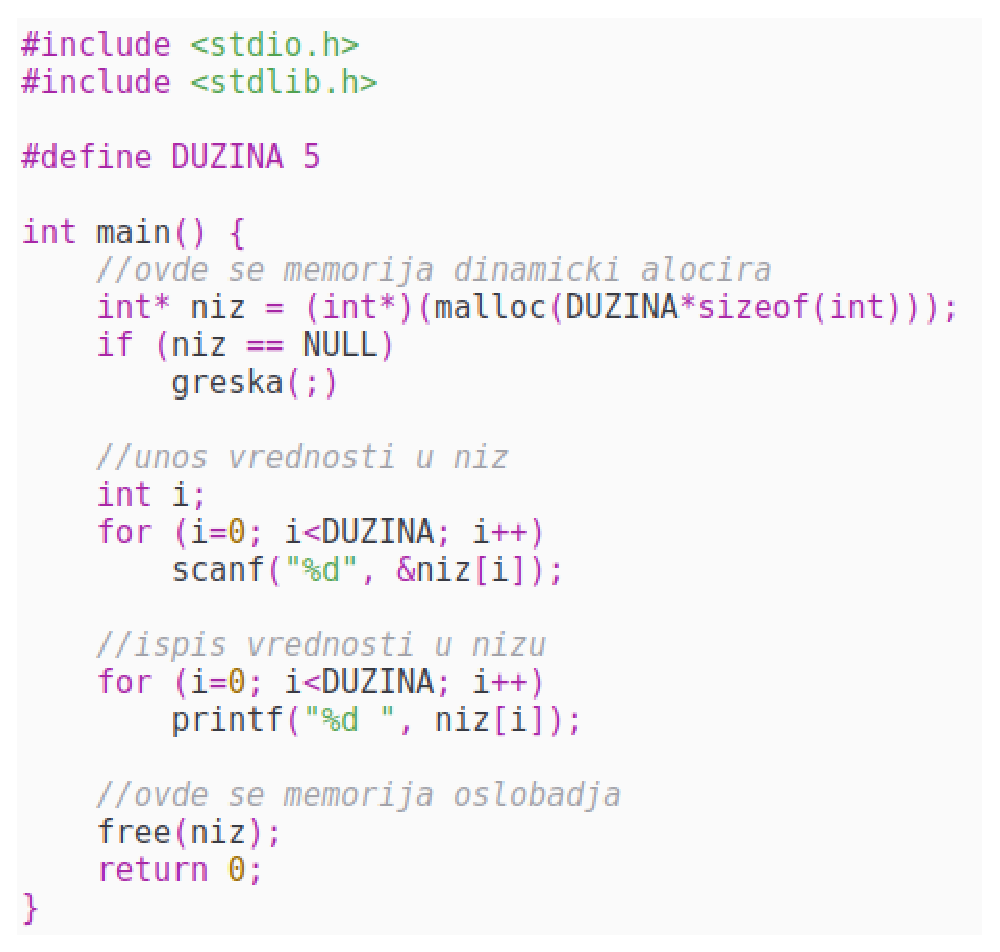
\includegraphics[scale=0.4]{c_kod_dinamicka_alokacija.eps}
\end{center}
\caption{Kod programa napisan u jeziku C}
\label{fig:ckod}
\end{figure}

Na slici \ref{fig:ckod} prikazan je način na koji se u jeziku C obično sprovodi kreiranje, pristupanje, i oslobađanje dinamički alocirane memorije.
\end{primer}

\begin{primer} Program koji učitava vrednosti u dinamički alociran niz, a potom ih ispisuje, napisan u jeziku C++.

\begin{figure}[h!]
\begin{center}
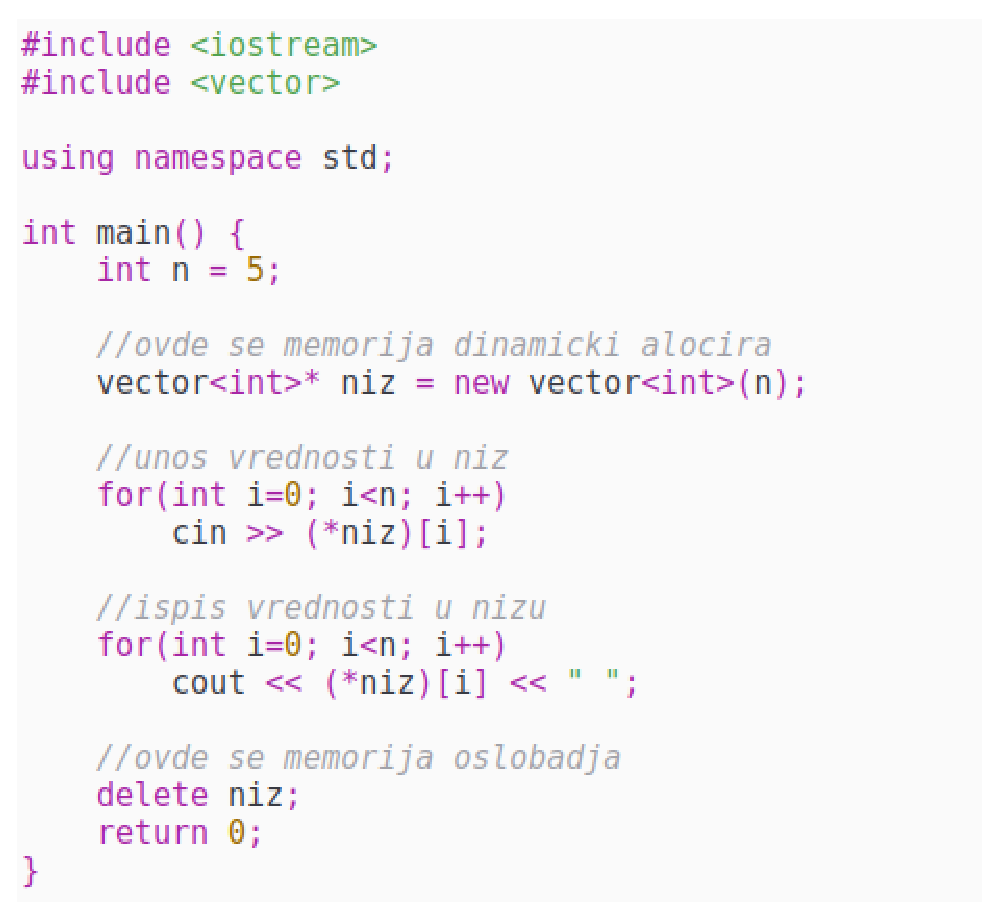
\includegraphics[scale=0.4]{cpp_kod_dinamicka_alokacija.eps}
\end{center}
\caption{Kod programa napisan u jeziku C++}
\label{fig:cppkod}
\end{figure}

Na slici \ref{fig:cppkod} prikazan je način na koji se u jeziku C++ obično sprovodi kreiranje, pristupanje, i oslobađanje dinamički alocirane memorije.
\end{primer}

Način na koji se manipuliše dinamički alociranom memorijom potpuno je analogan koršćenom u jeziku C, na slici \ref{fig:ckod}, mada je jednostavnija sintaksa jezika C++ često lakša za upotrebu u složenijim slučajevima.


\subsection{Upravljanje izuzecima}

U standardnoj biblioteci jezika C ne postoji implementiran sistem za upravljanje greškama. To znači da je ostavljeno programeru da sam dizajnira svoj sistem koji bi se time bavio. Česta posledica ovoga je kod sa velikim brojem uslovnih grananja u svrhu provere različitih grešaka, što čini kod sporijim i manje čitljivim.

Iz ovih razloga, programski jezik C++ uvodi upravljanje grešaka kroz ključne reči \emph{try, throw} i \emph{catch}. Ideja je, da se u \emph{try}-bloku nalazi kod u kojem očekujemo greške, tj. izuzetke, nakon kojeg sledi bar jedan \emph{catch}-blok koji se izvršava ako je pronađen odgovarajući izuzetak. Unutar \emph{try}-bloka se na mestu pronađene greške nalazi ključna reč \emph{throw}, koja obustavlja dalje izvršavanje bloka, i ,,baca'', tj. daje informaciju, obično vrednost prostog tipa, ili, češće, objekat sa informacijama o nastalom izuzetku. Na osnovu tipa koji je ,,bačen'', pronalazi se odgovarajući \emph{catch}-blok se izvršava, tj. on ,,hvata'' odgovarajući izuzetak.

Ovakav pristup upravljanju izuzecima ima dve značajne prednosti. Prvo, kod koji se bavi izuzecima je odvojen od glavnog koda, što poboljšava razumljivost. Drugo, omogućeno je programeru da bira, koje će izuzetke obraditi. Naime, pošto je moguće pri različitim izuzecima ,,baciti'' različite tipove vrednosti, moguće je birati koje tipove vrednosti ili klase objekata obrađivati zasebno, a koje ne.

% možda primer koda

\section{Gde se C danas koristi}
Iako je programski jezik C bio namenjen pre svega pisanju sistemskog softvera, usled njegove velike popularnosti koristio se i kao jezik opšte namene. Vremenom su mnoge uloge koje je programski jezik C imao od svog nastanka 1972. godine preuzeli drugi, moderniji programski jezici. Međutim i danas 50 godina nakon svog nastanka programski jezik C ima veliku popularnost. Neke od oblasti primena programskog jezika C danas su:
\begin{itemize}
    \item operativni sistemi;
    \item programiranje ugrađenih sistema;
    \item izrada kompilatora i interpretatora;
    \item u obrazovanju.
\end{itemize}
C programski jezik imam najveću primenu u pisanju programa \textquote{bliskih hardveru}. To nije slučajnost budući da je jezik od početka tako dizajniran. Prema rečima Brajana Kernigena\footnote{Brian W. Kernighan (1942), kanadski informatičar} i Denis Ričija \textquote{C je jezik dosta {\em niskog nivoa}. Ta karakterizacija nije pežorativna; to samo znači da se C nosi sa objektima na sličan način kao i većina računara}. Razlog što je C uspešan u oblastima kao što su sistemsko programiranje i programiranje ugrađenih sistema je u tome što nudi mnoge prednosti jezika višeg nivoa uz jako malo žrtvovanja u odnosu na programiranje na asembleru. Neke od prednosti u odnosu na asembler su lakše i udobnije pisanje čitkog i kompaktnog koda na jeziku koji poznatom velikom broju programera kao i visok nivo prenosivosti koda. C kompilatori su dostupni za većinu današnjih procesora, što oslobađa programera od brige o implementaciji konkretne procesorske arhitekture. Sa druge strane u odnosu na većinu viših programskih jezika, C nudi visok nivo kontrole nad hardverom i veoma visoku efikasnost u izvršavanju programa\cite{Programming Embedded Systems}.

\subsection{Programiranje ugrađenih sistema}
Ugrađeni sistem je kombinacija računarskog hardvera i softvera kao i drugih mehaničkih i električnih
delova koji ima neku određenu funkciju. Za razliku od ličnih računara, koji imaju mnoštvo različitih funkcija i primena, ugrađeni sistemi obično imaju jednu konkretnu svrhu često kao deo nekog većeg sistema. Primeri su mnogobrojni uređaji u automobilima (npr. čipovi koji kontrolišu rad ABS sistema), jednostavni digitalni časovnici, razni uređaji u  domaćinstvu i drugi. Budući da su mogućnosti takvih sitema često jako ograničene u smislu memorije i procesorske snage, pre svega radi uštede na ceni i dimenzijama uređaja, efikasnost programa je jako bitna. Upravo zbog toga je C pogodan za tu namenu više nego i jedan drugi jezik. Osim C-a se često se koriste i asembler i C++, međutim prednosti koje C++ donosi često nisu vredne gubitaka na efikasnosti osim kod jako velikih razvojnih timova\cite{Programming Embedded Systems}.

\subsection{Sistemsko programiranje}Sistemsko programiranje, odnosno programiranje operativnih sistema takođe zahteva jezik blizak hardveru. C programski jezik je upravo dizajniran za potrebe sistemskog programiranja i to u okviru operativnog sistema Unix. Među modernim operativnim sistemima C se najviše vezuje za Linux operativni sistem, ali većina popularnih operativnih sistema je barem značajnim delom pisana u jeziku C. O značaju C programskog jezika u sistemskom programiranju govori podatak da je u Arch Linux distrubuciji Linux operativnog sistema (poznatoj po minimalnoj instalaciji), preko 97\% programskog koda jezgra napisano u jeziku C kao i najveći deo od 27 osnovnih paketa koji omogućavaju osnovnu instalaciju sistema\cite{relevanceofc}.

\section{Gde se C++ danas koristi}

Iz činjenica da je C++, zbog svoje bliskosti sa hardverom, prilično brz i efikasan jezik, a opet jednostavniji za implementaciju velikih projekata nego C, rezultovalo je to da je veliki deo za računar zahtevnog aplikativnog softvera pisan u jeziku C++. Veliki deo softvera za grafičke obrade je pisan u jeziku C++ (Adobe Photoshop, Adobe Illustrator, itd.), kao i veliki broj video igara (Unreal engine). Takođe, C++ je našao primenu u veb pregledačima kao što su Mozilla Firefox i Google Chrome, ali i softveru za rad sa bazama podataka MySQL. Kompilatori za neke više programske jezike, kao što su Java i C\# su takođe pravljeni u jeziku C++.

\section{Zaključak}
\label{sec:zakljucak}
C i C++ su jezici sa velikim značajem, kako u istoriji programiranja tako i u današnjoj upotrebi. C je svoju upotrebu pronašao u programiranju niskog nivoa i izradi jezgara operativnih sistema, dok je C++ korišćen u softveru kome je neophodna grafika, kao što su internet pregledači, programi za obrađivanje fotografija i video zapisa i video igrama. Prilikom započinjanja novog projekta potrebno je uzeti sve navedene razlike u obzir i napraviti odluku koji od ova dva stara programska jezika, koji su i dalje u širokoj upotrebi, treba iskoristiti.


\addcontentsline{toc}{section}{Literatura}
\appendix

\iffalse
\bibliography{seminarski}
\bibliographystyle{plain}
\fi

\begin{thebibliography}{9}

\bibitem{programiranje1} F. Marić, P. Janičić. \emph{Programiranje 1}. Matematički fakultet, Beograd, 2015.

\bibitem{programiranje2} P. Janičić, F. Marić. \emph{Programiranje 2}. Matematički fakultet, Beograd, 2022.

\bibitem{exceptions} A. Koenig, B. Stroustrup. \emph{Exception Handling for C++}. The Evolution of C++: Language Design in the Marketplace of Ideas, 1993.

\bibitem{history} B. Stroustrup. \emph{A history of C++ 1979--1991}. History of programming languages---II. 1996. 699-769.

\bibitem{Programming Embedded Systems} M. Barr, A. Massa. \emph{Programming Embedded Systems: With C and GNU Development Tools, 2nd Edition}. O'Reilly Media , 2006
\bibitem{relevanceofc}The relevance of C in systems programming. LupLab  Department of Computer Science, at the University of California, Davis on-line at: https://luplab.cs.ucdavis.edu/2021/03/08/the-relevance-of-c-in-systems-programming.html
\bibitem{efficiency} R. Pereira, M. Couto, F. Ribeiro, R. Rua, J. Cunha, J. Paulo Fernandes, J. Saraiva.  \emph{Energy Efficiency across Programming Languages}. SLE 2017: Proceedings of the 10th ACM SIGPLAN International Conference on Software Language Engineering, Pages 256–267, October 2017.
\end{thebibliography}
\end{document}
